%%%%%%%%%%%%%%%
%
% $Autor: Wings $
% $Datum: 2020-01-29 07:55:27Z $
% $Pfad: Nano33BLESense.tex $
% $Version: 1785 $
%
%
%%%%%%%%%%%%%%%


%todo citatzions in correct manner
%source: {\tiny Quelle: \url{https://www.arduino.cc/pro/tutorials/portenta-h7}}



%todo GitLab\ToDo\TinyML
% TinyML Seite 222

%source: \url{https://www.reichelt.de/de/de/arduino-nano-33-ble-sense-nrf52840-ohne-header-ard-nano-33bles-p261306.html?PROVID=2788&gclid=Cj0KCQjwna2FBhDPARIsACAEc_Uui0sowk2McNvt69o9wzQJtqHWW2n5l_OHng2pSRcmfYqUsiosbdUaAp47EALw_wcB&&r=1}


\chapter{Arduino Nano 33 BLE Sense Lite}


Arduino ist eine Open-Source-Elektronikplattform, die auf leicht zugänglicher Hardware und Software basiert. Sie stellt Mikrocontroller- und Mikroprozessorkits bereit, mit denen sich sowohl digitale als auch analoge Anwendungen realisieren lassen. Der Mikrocontroller – oft als eingebetteter Mini-Computer auf dem Arduino-Board bezeichnet – benötigt üblicherweise zusätzliche elektronische Bauteile wie Dioden, Widerstände, Kondensatoren oder Transistoren, um Spannungen und Ströme korrekt zu steuern.\\

Das Arduino-Team hat jedoch eine benutzerfreundliche Umgebung geschaffen, die viele dieser elektronischen Komplexitäten abstrahiert. Statt komplexer Schaltungen genügt es, das Board mit der vorgesehenen Spannung zu versorgen, das gewünschte Programm zu schreiben und es innerhalb weniger Sekunden auf den Mikrocontroller zu übertragen. Dadurch wird die gesamte Hardwarefunktionalität durch Softwaresteuerung zugänglich gemacht, ohne tiefgreifende Elektronikkenntnisse zu erfordern.\\

Durch den technologischen Fortschritt in der Halbleiter- und Elektronikindustrie lassen sich viele Steuerungsaufgaben heute mithilfe kompakter Mikrocontroller lösen – anstelle mechanischer oder elektromechanischer Schalter. Allen Arduino-Boards ist gemeinsam, dass sie einen Mikrocontroller enthalten – einen kleinen, programmierbaren Rechner, der sich ideal für Anwendungen im Bereich des Edge Computings eignet
\cite{Arduino:2021b}.


\section{Arduino Nano 33 BLE Sense}

Die Arduino Nano-Familie umfasst eine Reihe kompakter Boards mit vielfältigen Funktionen – vom preisgünstigen Einstiegsmodell bis hin zu leistungsfähigeren Varianten wie dem Nano 33 BLE Sense oder dem Nano RP2040 Connect, die mit integrierten Bluetooth- bzw. Wi-Fi-Modulen ausgestattet sind. Darüber hinaus verfügen diese Boards über eine Reihe eingebetteter Sensoren, etwa für Temperatur, Luftfeuchtigkeit, Luftdruck, Gestenerkennung, Geräuscherfassung und weitere Umgebungsparameter. Sie unterstützen sowohl die Programmierung in C/C++ als auch in MicroPython und ermöglichen die Einbindung von Machine-Learning-Anwendungen.\\

Das Arduino Nano 33 BLE Sense ist ein leistungsfähiges Modell dieser Serie. Es kombiniert Bluetooth Low Energy (BLE) Kommunikation mit einer umfangreichen Sensorausstattung und basiert auf dem NINA B306 Modul, das für BLE- und Bluetooth 5.0-Verbindungen ausgelegt ist – dem aktuellen Standard für energiesparende drahtlose Kommunikation. Als zentraler Mikrocontroller kommt ein Nordic nRF52840 zum Einsatz, ausgestattet mit einem Cortex-M4F-Prozessor. Aufgrund seiner kompakten Bauform, der reduzierten Leistungsaufnahme und seiner umfangreichen Sensorik eignet sich das Board besonders für energieeffiziente, interaktive und tragbare Anwendungen.\\

Die Modellbezeichnung Arduino Nano 33 BLE Sense verweist bereits auf zentrale Eigenschaften: Die Bezeichnung „Nano“ beschreibt das kompakte Format des Boards, „33“ steht für die Betriebsspannung von 3,3 Volt, „BLE“ kennzeichnet die integrierte Bluetooth-Low-Energy-Funktionalität, und „Sense“ weist auf die Vielzahl integrierter Sensoren hin, darunter Beschleunigungs-, Lage-, Magnetfeld-, Temperatur-, Feuchtigkeits- und Luftdrucksensoren, ein Näherungs-, Farb- und Gestensensor sowie ein eingebettetes Mikrofon.\\

Für Anwendungen im Bereich Objekterkennung, Farbanalyse oder Gestensteuerung kann das Arduino Nano 33 BLE Sense mit dem Kamera-Shield Arducam OV2640 kombiniert werden. Dieses Kameramodul erweitert die Sensorik des Boards um Bildverarbeitungsfunktionen und eignet sich besonders für KI- und Machine-Learning-Anwendungen. Durch die Installation geeigneter Bibliotheken lassen sich alle Sensoren und das Kameramodul direkt über die Arduino-Entwicklungsumgebung ansprechen und in intelligente Systeme integrieren.


%Abbildung noch mal kontrollieren!!!
Die folgende Abbildung ~\ref{ArduinoNano33} zeigt einen Arduino Nano 33 BLE Sense Revision 2, zu sehen ist die kompackte Bauform.

\begin{center}

%    \includegraphics[width=0.9\linewidth]{Arduino/ArduinoNano33BLESense}
%    
\includegraphics[width=0.45\linewidth]{Nano33BLESense/ArduinoNano33BLESenseTopology}
   

\begin{tikzpicture}
  \ArduinoNanoBLESenseRev
\end{tikzpicture}
    
%    
%    \includegraphics[width=0.45\linewidth]{Arduino/ArduinoNano33BLESense2}
% 
 
    
    \captionof{figure}{Arduino Nano 33 BLE Sense Rev. 2, see \href{https://store.arduino.cc/arduino-nano-33-ble-sense}{Arduino Store}} 
    \label{ArduinoNano33}
\end{center}


Das kompakte und zuverlässige Arduino Nano 33 BLE Sense Board basiert auf dem NINA B306 Modul, das für Bluetooth Low Energy (BLE) und Bluetooth 5 Kommunikation ausgelegt ist. Dieses Modul wiederum verwendet den Nordic nRF52840 Prozessor, der mit einem leistungsfähigen Cortex-M4F-Kern ausgestattet ist. Die Architektur des Boards ist vollständig kompatibel mit der Arduino IDE, sowohl in der Online- als auch in der Offline-Version. Das Arduino Nano 33 BLE Sense integriert eine Vielzahl von Sensoren auf kleinstem Raum und eignet sich daher hervorragend für kompakte, sensorbasierte Anwendungen
\cite{Arduino:2021}.\\

Zu den auf dem Board verbauten Sensoren gehören der ADPS-9960, der Umgebungslicht, RGB-Farbe, Näherung und Gesten erfassen kann, sowie der LSM9DS1, der als System-in-Package eine dreiachsige Beschleunigungserfassung, ein Gyroskop und ein Magnetometer kombiniert. Der LPS22HB misst den Luftdruck und die Umgebungstemperatur, während der HTS221 für die Erfassung der relativen Luftfeuchtigkeit zuständig ist. Zusätzlich ist mit dem MP34DT05-A ein digitales Mikrofon integriert, das Audiosignale erfassen kann. Die Bluetooth-Kommunikation wird über das bereits erwähnte NINA B306 Modul abgewickelt, wodurch drahtlose Datenübertragung mit geringem Energieverbrauch möglich wird. Mit dieser umfangreichen Ausstattung lassen sich komplexe IoT- und KI-Projekte auf kleinstem Raum realisieren.\\



\subsection{Arduino Nano 33 BLE Sense Lite}

\chapter{Arduino Tiny Machine Learning Kit}
Das Arduino Tiny Machine Learning Kit ist eine leistungsfähige Entwicklungsplattform, die es ermöglicht, Machine-Learning-Modelle direkt auf energieeffizienter Mikrocontroller-Hardware auszuführen. Im Mittelpunkt des Kits steht das Arduino Nano 33 BLE Sense Lite Board, das eine Vielzahl integrierter Sensoren für Beschleunigung, Temperatur, Luftdruck, Geräusche, Gesten und vieles mehr beinhaltet. \cite{Reichelt_ArduinoKit:2025} \\
Enthalten sind:
\begin{itemize}
	\item Arduino Nano 33 BLE Sense Lite
	\item Kameramodul (OV7675)
	\item Arduino Tiny Machine Learning Shield
	\item USB-A-auf-USB-Micro-Verbindungskabel
\end{itemize}

\begin{center}
	
\includegraphics[width=0.75\textwidth]{Nano33BLESense/TinyMLKit/TinyMachineLearningKit.png}
	\captionof{figure}{Arduino Tiny Machine Learning Kit\cite{Reichelt_ArduinoKit:2025}}
	\label{ArduinoKit}
\end{center}

\section{Arduino Nano 33 BLE Sense Lite}
\label{chap:ArduinoNano33BLESenseLite}
Das Arduino® Nano 33 BLE Sense ist ein kompakt gebautes Entwicklungsboard, das mit dem NINA B306 Funkmodul ausgestattet ist. Dieses Modul basiert auf dem Nordic nRF52840 Mikrocontroller und nutzt einen leistungsstarken Arm® Cortex-M4F® Prozessor. Zusätzlich verfügt es über einen integrierten Kryptografie-Chip, der eine sichere Speicherung von Zertifikaten und vorab geteilten Schlüsseln ermöglicht. Für Anwendungen im Bereich Bewegungserkennung bietet das Board außerdem eine 9-Achsen-Inertialsensorik (IMU). Die Platine kann flexibel entweder als steckbares Bauteil mit montierten Stiftleisten oder durch direktes Verlöten der castellierten Kontaktflächen auf einer Leiterplatte verwendet werden.\cite{Arduino:2025}\\
Das Arduino Nano 33 BLE Sense besitzt, wie alle Modelle der Nano-Serie, kein integriertes Ladesystem. Die Energieversorgung erfolgt wahlweise über die USB-Schnittstelle oder über die an den Stiftleisten verfügbaren Versorgungsanschlüsse.\cite{Arduino:2025}\\
Zu beachten ist, dass dieses Board ausschließlich mit 3,3-Volt-Pegeln an seinen Ein- und Ausgängen arbeitet. Eine direkte Verbindung von 5-Volt-Signalen kann die Schaltung irreparabel beschädigen.\cite{Arduino:2025} \\
Anders als bei älteren Arduino Nano-Versionen, bei denen der 5V-Pin eine stabile 5V-Versorgung bereitstellt, ist dieser Anschluss beim Nano 33 BLE Sense nicht als Spannungsquelle nutzbar. Er ist lediglich intern mit dem USB-Eingang verbunden und führt nur dann Spannung, wenn das Board per USB mit Strom versorgt wird.\cite{Arduino:2025}

\subsection{Pinbelegung}
Die exakte Zuordnung der verfügbaren Pins des Arduino Nano 33 BLE Sense wird in Abbildung~\ref{ArduinoPinbelegung} grafisch dargestellt. Eine detaillierte Übersicht über die Funktionen, Signaltypen und Anschlussmöglichkeiten der einzelnen Pins liefert Tabelle~\ref{tab:Pinbelegung}. Diese Informationen sind essenziell für die korrekte Anbindung externer Komponenten und die Planung von Schaltungen.
\begin{center}
	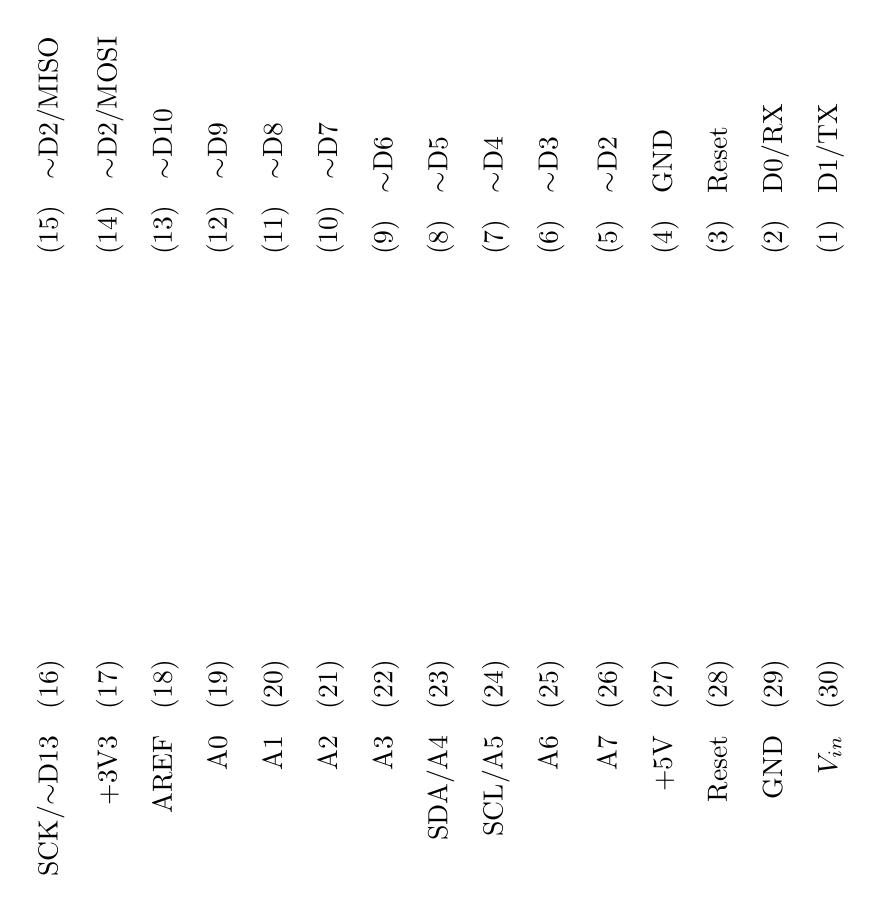
\begin{tikzpicture}
		
		\ArduinoNanoBLESenseRev
		
		\node[rotate=90,right] (Pin1) at (11.2,4.9) {(1) \; D1/TX};
		\node[rotate=90,right] (Pin2) at (10.5,4.9) {(2) \; D0/RX};
		\node[rotate=90,right] (Pin3) at (9.8,4.9) {(3) \; Reset};
		\node[rotate=90,right] (Pin4) at (9.1,4.9) {(4) \; GND};
		\node[rotate=90,right] (Pin5) at (8.4,4.9) {(5) \; $\sim$D2};
		\node[rotate=90,right] (Pin6) at (7.65,4.9) {(6) \; $\sim$D3};
		\node[rotate=90,right] (Pin7) at (6.95,4.9) {(7) \; $\sim$D4};
		\node[rotate=90,right] (Pin8) at (6.25,4.9) {(8) \; $\sim$D5};
		\node[rotate=90,right] (Pin9) at (5.55,4.9) {(9) \; $\sim$D6};
		\node[rotate=90,right] (Pin10) at (4.85,4.9) {(10) \; $\sim$D7};
		\node[rotate=90,right] (Pin11) at (4.15,4.9) {(11) \; $\sim$D8};
		\node[rotate=90,right] (Pin12) at (3.45,4.9) {(12) \; $\sim$D9};
		\node[rotate=90,right] (Pin13) at (2.75,4.9) {(13) \; $\sim$D10};
		\node[rotate=90,right] (Pin14) at (2.05,4.9) {(14) \; $\sim$D2/MOSI};
		\node[rotate=90,right] (Pin15) at (1.3,4.9) {(15) \; $\sim$D2/MISO};
		
		
		\node[rotate=90,left] (Pin30) at (11.2,-0.0) { $V_{in}$ \; (30)};
		\node[rotate=90,left] (Pin1) at (10.5,-0.0) {GND \; (29)};
		\node[rotate=90,left] (Pin2) at (9.8,-0.0) {Reset \; (28)};
		\node[rotate=90,left] (Pin3) at (9.1,-0.0) {+5V \; (27)};
		\node[rotate=90,left] (Pin4) at (8.4,-0.0) {A7 \; (26)};
		\node[rotate=90,left] (Pin5) at (7.65,-0.0) {A6 \; (25)};
		\node[rotate=90,left] (Pin6) at (6.95,-0.0) {SCL/A5 \; (24)};
		\node[rotate=90,left] (Pin7) at (6.25,-0.0) {SDA/A4 \; (23)};
		\node[rotate=90,left] (Pin8) at (5.55,-0.0) {A3 \; (22)};
		\node[rotate=90,left] (Pin9) at (4.85,-0.0) {A2 \; (21)};
		\node[rotate=90,left] (Pin10) at (4.15,-0.0) {A1 \; (20)};
		\node[rotate=90,left] (Pin11) at (3.45,-0.0) {A0 \; (19)};
		\node[rotate=90,left] (Pin12) at (2.75,-0.0) {AREF \; (18)};
		\node[rotate=90,left] (Pin13) at (2.05,-0.0) {+3V3 \; (17)};
		\node[rotate=90,left] (Pin14) at (1.3,-0.0) {SCK/$\sim$D13 \; (16)};
		
	\end{tikzpicture}
	\captionof{figure}{Arduino Pinbelegung}
	\label{ArduinoPinbelegung}
\end{center}

\begin{longtable}{|c|p{2cm}|c|p{6.5cm}|}
	\caption{Pinbelegung des Arduino Nano 33 BLE Sense\cite{Arduino:2025}}
	\label{tab:Pinbelegung} \\
	\hline
	\textbf{PIN} & \textbf{Funktion} & \textbf{Typ} & \textbf{Beschreibung} \\
	\hline
	\endfirsthead
	\hline
	\textbf{PIN} & \textbf{Funktion} & \textbf{Typ} & \textbf{Beschreibung} \\
	\hline
	\endhead
	\hline
	\endfoot
	
	\hline
	1 & D13 & Digital & GPIO\\
	\hline
	2 & +3V3 & Power Out & Intern erzeugte Stromausgabe an externe Geräte \\
	\hline
	3 & AREF & Analog & Analoge Referenz; kann als GPIO verwendet werden \\
	\hline
	4 & A0/DAC0 & Analog & ADC-Eingang/DAC-Ausgang, kann als GPIO verwendet werden\\
	\hline
	5 & A1 & Analog & ADC-Eingang; kann als GPIO verwendet werden \\
	\hline
	6 & A2 & Analog & ADC-Eingang; kann als GPIO verwendet werden\\
	\hline
	7 & A3 & Analog & ADC-Eingang; kann als GPIO verwendet werden \\
	\hline
	8 & A4/SDA & Analog & ADC-Eingang; I2C SDA; kann als GPIO verwendet werden \\
	\hline
	9 & A5/SCL & Analog & ADC-Eingang; I2C SCL; kann als GPIO verwendet werden \\
	\hline
	10 & A6 & Analog & ADC-Eingang; kann als GPIO verwendet werden \\
	\hline
	11 & A7 & Analog & ADC-Eingang; kann als GPIO verwendet werden \\
	\hline
	12 & VUSB & Power In/Out & Normalerweise NC; kann durch Kurzschließen eines Jumpers an den VUSB-Pin des USB-Anschlusses angeschlossen werden \\
	\hline
	13 & RST & Digital In & Aktiv-Low-Reset-Eingang (Duplikat von Pin 18)\\
	\hline
	14 & GND & Power & Strom Masse \\
	\hline
	15 & VIN & Power In & VIN Stromeingang \\
	\hline
	16 & TX & Digital & USART TX; Kann als GPIO verwendet werden \\
	\hline
	17 & RX & Digital & USART RX; Kann als GPIO verwendet werden \\
	\hline
	18 & RST & Digital & Aktiv-Low-Reset-Eingang (Duplikat von Pin 13) \\
	\hline
	19 & GND & Power & Strom Masse \\
	\hline
	20 & D2 & Digital & GPIO \\
	\hline
	21 & D3/PWM & Digital & GPIO; kann als PWM verwendet werden \\
	\hline
	22 & D4 & Digital & GPIO \\
	\hline
	23 & D5/PWM & Digital & GPIO; kann als PWM verwendet werden \\
	\hline
	24 & D6/PWM & Digital & GPIO; kann als PWM verwendet werden \\
	\hline
	25 & D7 & Digital & GPIO \\
	\hline
	26 & D8 & Digital & GPIO \\
	\hline
	27 & D9/PWM & Digital & GPIO; kann als PWM verwendet werden \\
	\hline
	28 & D10/PWM & Digital & GPIO; kann als PWM verwendet werden \\
	\hline
	29 & D11/MOSI & Digital & SPI MOSI; kann als GPIO verwendet werden \\
	\hline
	30 & D12/MISO & Digital & SPI MISO; kann als GPIO verwendet werden \\
	\hline
	
\end{longtable}

\subsection{Mechanik}
Formfaktor: Der Arduino Nano 33 BLE Sense hat einen kleinen Formfak
tor, der typischerweise etwa 45mm x 18mm misst, wobei Toleranzen von
etwa +/- 1mm möglich sind. Montagemöglichkeiten: Die Platine verfügt
über Bohrungen mit einem Durchmesser von etwa 3mm, wobei Toleranzen
von +/- 0,5mm möglich sind. \cite{Arduino:2025}

\subsection{Elektronik}
Prozessoreinheit: Der Arduino Nano 33 BLE Sense wird von einem 64 MHz
Arm Cortex-M4F Prozessor angetrieben, wobei die Taktfrequenz um bis
zu +/- 5 MHz variieren kann. NINA B306 Modul: Das integrierte NINA
B306 Modul bietet Bluetooth 5-Konnektivität mit einer Sendeleistung
von +8 dBm und Empfindlichkeit von-95 dBm, wobei Toleranzen von
+/- 1 dB möglich sind. \cite{Arduino:2025}

\subsection{Verbaute Sonsoren}

\textbf{LSM9DS1 - Trägheitssensor:} Die Sensordaten haben eine Genauigkeit
von etwa +/- 5 Prozent und eine Prozentual mögliche Messbereichs
toleranz von +/- 2 Prozent.
\\\\
\textbf{LPS22HB - Drucksensor:} Der Drucksensor hat eine Genauigkeit von
etwa +/- 0,5 hPa und eine Temperaturgenauigkeit von etwa +/
0,2°C.
\\\\
\textbf{HTS221 - Feuchtigkeitssensor:} Die relative Feuchtigkeitsmessung hat
eine Genauigkeit von etwa +/- 5 Prozent und eine Temperaturge
nauigkeit von etwa +/- 0,5°C.
\\\\
\textbf{APDS-9960 - Näherungs- und RGB-Sensor:} Die Näherungssensorgenau
igkeit beträgt etwa +/- 2 mm, die RGB-Farberkennung hat eine
Genauigkeit von etwa +/- 5 Prozent.
\\\\
\textbf{MP34DT05 - Digitales Mikrofon:} Die Genauigkeit des digitalen Mikro
fons beträgt etwa +/- 2 dB.
\\\\
\textbf{ATECC608A - Kryptografischer Co-Prozessor:} Die kryptografische Funk
tion hat eine Genauigkeit von etwa +/- 1 Bit.
\\\\
\textbf{MPM3610 - DC-DC-Wandler:} Die Effizienz des DC-DC-Wandlers kann
um bis zu +/- 5 Prozent variieren.
\\
\begin{center}
	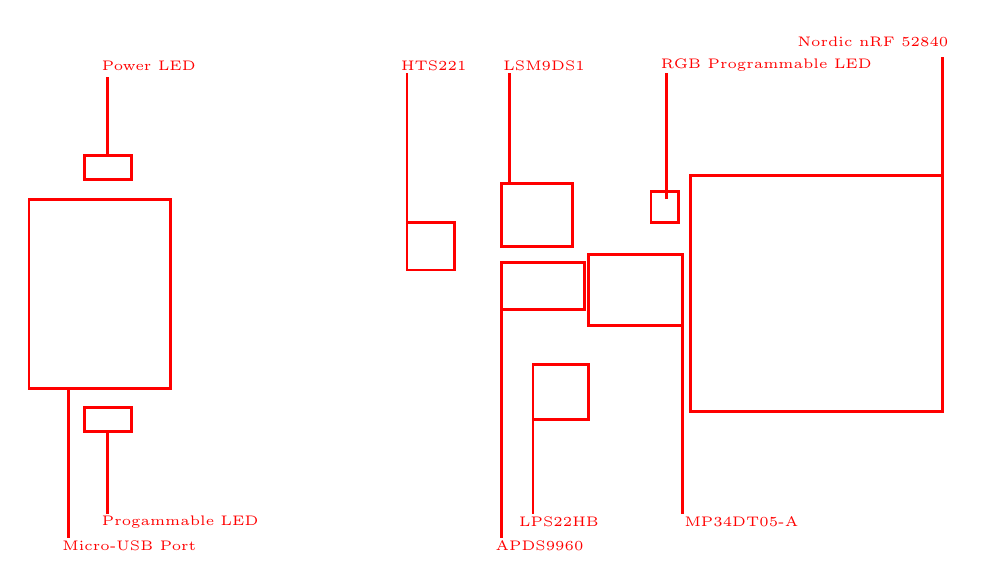
\begin{tikzpicture}
		\ArduinoNanoBLESenseOne
		
		\node[right](LEDPower) at (0.5,5.4){\textcolor{red}{\tiny Power LED}};
		\draw[line width=1pt,red]  (0.7,5.25) -- (0.7,4.25);
		\draw[line width=1pt,red] (0.4,4.25) -- (1.0, 4.25) -- (1.0,3.95) -- (0.4,3.95) -- cycle;
		
		\node[right](HTS) at (4.3,5.4){\textcolor{red}{\tiny HTS221}};
		\draw[line width=1pt,red]  (4.5,3.4) -- (4.5,5.3);
		\draw[line width=1pt,red] (4.5,3.4) -- (5.1, 3.4) -- (5.1,2.8) -- (4.5,2.8) -- cycle;
		
		\node[right](LSM9DS1) at (5.6,5.4){\textcolor{red}{\tiny LSM9DS1}};
		\draw[line width=1pt,red]  (5.8,3.9) -- (5.8,5.3);
		\draw[line width=1pt,red] (5.7,3.9) -- (6.6, 3.9) -- (6.6,3.1) -- (5.7,3.1) -- cycle;
		
		\node[right](RGB) at (7.6,5.4){\textcolor{red}{\tiny RGB Programmable LED}};
		\draw[line width=1pt,red]  (7.8,3.7) -- (7.8,5.3);
		\draw[line width=1pt,red] (7.6,3.8) -- (7.95, 3.8) -- (7.95,3.4) -- (7.6,3.4) -- cycle;
		
		\node[right](APD) at (5.5,-0.7){\textcolor{red}{\tiny APDS9960}};
		\draw[line width=1pt,red]  (5.7,2.3) -- (5.7,-0.6);
		\draw[line width=1pt,red] (5.7,2.9) -- (6.75, 2.9) -- (6.75,2.3) -- (5.7,2.3) -- cycle;
		
		\node[right](MP) at (7.9,-0.4){\textcolor{red}{\tiny MP34DT05-A}};
		\draw[line width=1pt,red]  (8,2.1) -- (8,-0.3);
		\draw[line width=1pt,red] (6.8,3.0) -- (8, 3.0) -- (8,2.1) -- (6.8,2.1) -- cycle;
		
		\node[left](HTS) at (11.5,5.7){\textcolor{red}{\tiny Nordic nRF 52840}};
		\draw[line width=1pt,red]  (11.3,4) -- (11.3,5.5);
		\draw[line width=1pt,red] (8.1,4) -- (11.3,4) -- (11.3,1) -- (8.1,1) -- cycle;
		
		\node[right](LPS) at (5.8,-0.4){\textcolor{red}{\tiny LPS22HB}};
		\draw[line width=1pt,red]  (6.1,1.0) -- (6.1,-0.3);
		\draw[line width=1pt,red] (6.1,0.9) -- (6.1,1.6) -- (6.8,1.6) -- (6.8,0.9) -- cycle;
		
		\node[right](LEDPower) at (0.5,-0.4){\textcolor{red}{\tiny Progammable LED}};
		\draw[line width=1pt,red]  (0.7,0.75) -- (0.7,-0.3);
		\draw[line width=1pt,red] (0.4,0.75) -- (1.0, 0.75) -- (1.0,1.05) -- (0.4,1.05) -- cycle;
		
		\node[right](USB) at (0,-0.7){\textcolor{red}{\tiny Micro-USB Port}};
		\draw[line width=1pt,red]  (0.2,1.3) -- (0.2,-0.6);
		\draw[line width=1pt,red] (-0.3,1.3) -- (-0.3, 3.7) -- (1.5,3.7) -- (1.5,1.3) -- cycle;
		
		
	\end{tikzpicture}
	\captionof{figure}{Arduino Nano 33 BLE Sense Architektur}\label{ArduinoNano33BLESenseArchitecture}
\end{center}
The Tiny Machine Learning Kit contains only the Arduino Nano 33 BLE Sense Lite. \Mynote{citation}

\bigskip



\bigskip

The Arduino Nano 33 BLE Sense Lite differs only slightly from the Arduino Nano 33 BLE Sense Revision~1. The only difference between the two models is that the Lite version does not have the HTS221, the sensor for relative humidity and temperature. The LPS22HB sensor, which is on the board, is a pressure sensor, but it can also be used to measure the temperature. It is therefore not possible to measure humidity with the Arduino Nano 33 BLE Lite. To measure relative humidity, a separate sensor must be connected. The reason for this decision is that the Arduino company has difficulties maintaining the stock. \cite{Filipi:2022}




The figure~\ref{ArduinoNano33OneLite} presents the  layout of the Arduino Nano 33 BLE Lite,

\begin{center}
	
	%    \includegraphics[width=0.9\linewidth]{Arduino/ArduinoNano33BLESense}
	%    
\includegraphics[width=0.45\linewidth]{Nano33BLESense/ArduinoNano33BLESenseTopology}
	
	
    \begin{tikzpicture}
		\ArduinoNanoBLESenseLLite
	\end{tikzpicture}
	
	
	%\begin{tikzpicture}
	%  \ArduinoNanoBLESenseRev
	%\end{tikzpicture}
	
	%    
	%    \includegraphics[width=0.45\linewidth]{Arduino/ArduinoNano33BLESense2}
	% 
	
	
	\captionof{figure}[Arduino Nano 33 BLE Sense Lite]{Arduino Nano 33 BLE Sense Lite; the empty blavk square marks the postion of the missing sensor HTS221}
	%, see \href{https://store.arduino.cc/arduino-nano-33-ble-sense}{Arduino Store}}

\label{ArduinoNano33OneLite}
\end{center}


\section{On-Board Sensor Description}

Arduino Nano 33 BLE sense come up with the set of embed sensor on the board. The available embed sensors are commonly use for measuring both the analog and digital values around the sorrounding. Arduino Nano 33 BLE sense is very small 45mm $\times$ 18mm in size, which  makes it very usefull for Internet of things (IOT) and Artificial intelligence (AI) application as a embed device where space is the main constrained issue. It is low power consumption board and operate normally on 3.3 V, we can say that this small size low power consumption board can operate on small batteries even for many months. Due to on-board available sensor, the low power consumption and mini architecture we can use this nano board anywhere. The Arduino Nano 33 BLE Sense is a completely new board on a well-known form factor. For getting detail information about each component of Arduino Nano 33 BLE Sense and data sheets of each sensor the following links give us a detail information \cite{Arduino:2021}. The short description of each sensor are as follow. 

\begin{itemize}
    \item The ADPS-9960 is a digital proximity, ambient light, RGB and gesture sensor. it can measure the proximity distance, light, color and gestures when moving close with the borad.
    \item The sensor LSM9DS1 is a 9 axis \ac{imu} use as a accelerometre, gyroscope, and magnatometre, this 9 axis sensor is ideal for wearable devices.
    \item The sensor LPS22HB is a barometric pressure sensor, it measures the environmental pressure which is usefull for simple weather station monitoring. 
    \item The sensor HTS221 senses the relative humidity, and temperature, to get highly accurate measurements of the environmental conditions.
    \item The sensor MP34DT05 is the digital microphone. it is usefull for capturing, analyzing and detecting the sound in real time.
    \item The USB port allows you to connect  Arduino Nano 33 BLE sense to your machine.
    \item There are 3 different LEDs that can be accessed on the Nano BLE Sense: RGB Programmable LED , the built-in  orange Programmable LED and the Power LED.
    
\end{itemize}

The figure \ref{ArduinoNano33BLESenseArchitecture} show the embed sensors on the board, with powerful processor as compared to other arduino boards the nRF52840 from Nordic Semiconductors, a 32-bit ARM\textsuperscript{\textregistered} Cortex\textsuperscript{\texttrademark}-M4 CPU processor running at 64 MHz are as follow.

\begin{center}
  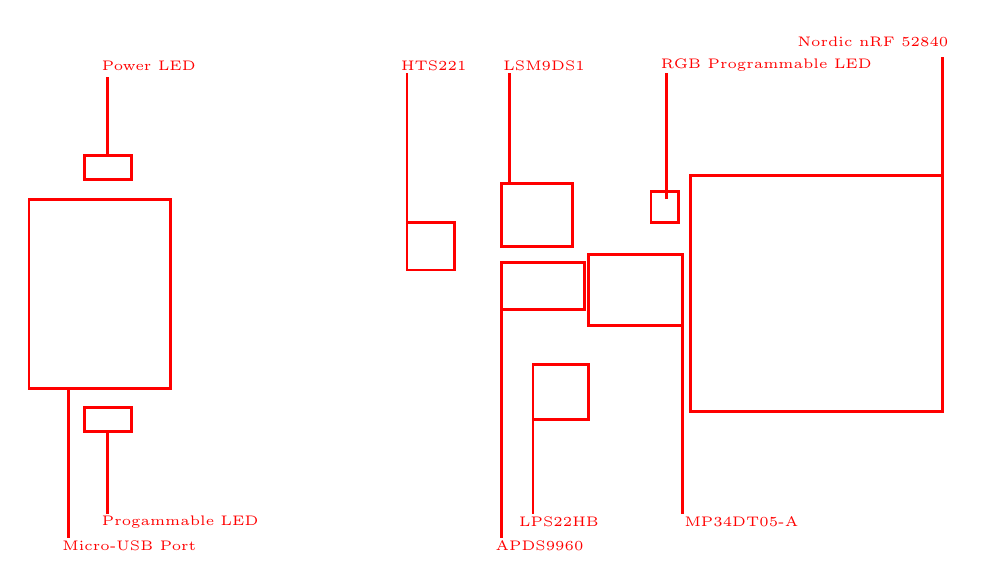
\begin{tikzpicture}
    \ArduinoNanoBLESenseOne

    \node[right](LEDPower) at (0.5,5.4){\textcolor{red}{\tiny Power LED}};
    \draw[line width=1pt,red]  (0.7,5.25) -- (0.7,4.25);
    \draw[line width=1pt,red] (0.4,4.25) -- (1.0, 4.25) -- (1.0,3.95) -- (0.4,3.95) -- cycle;
    
    \node[right](HTS) at (4.3,5.4){\textcolor{red}{\tiny HTS221}};
    \draw[line width=1pt,red]  (4.5,3.4) -- (4.5,5.3);
    \draw[line width=1pt,red] (4.5,3.4) -- (5.1, 3.4) -- (5.1,2.8) -- (4.5,2.8) -- cycle;

    \node[right](LSM9DS1) at (5.6,5.4){\textcolor{red}{\tiny LSM9DS1}};
    \draw[line width=1pt,red]  (5.8,3.9) -- (5.8,5.3);
    \draw[line width=1pt,red] (5.7,3.9) -- (6.6, 3.9) -- (6.6,3.1) -- (5.7,3.1) -- cycle;

    \node[right](RGB) at (7.6,5.4){\textcolor{red}{\tiny RGB Programmable LED}};
    \draw[line width=1pt,red]  (7.8,3.7) -- (7.8,5.3);
    \draw[line width=1pt,red] (7.6,3.8) -- (7.95, 3.8) -- (7.95,3.4) -- (7.6,3.4) -- cycle;
    
    \node[right](APD) at (5.5,-0.7){\textcolor{red}{\tiny APDS9960}};
    \draw[line width=1pt,red]  (5.7,2.3) -- (5.7,-0.6);
    \draw[line width=1pt,red] (5.7,2.9) -- (6.75, 2.9) -- (6.75,2.3) -- (5.7,2.3) -- cycle;

    \node[right](MP) at (7.9,-0.4){\textcolor{red}{\tiny MP34DT05-A}};
    \draw[line width=1pt,red]  (8,2.1) -- (8,-0.3);
    \draw[line width=1pt,red] (6.8,3.0) -- (8, 3.0) -- (8,2.1) -- (6.8,2.1) -- cycle;

    \node[left](HTS) at (11.5,5.7){\textcolor{red}{\tiny Nordic nRF 52840}};
    \draw[line width=1pt,red]  (11.3,4) -- (11.3,5.5);
    \draw[line width=1pt,red] (8.1,4) -- (11.3,4) -- (11.3,1) -- (8.1,1) -- cycle;
    
    \node[right](LPS) at (5.8,-0.4){\textcolor{red}{\tiny LPS22HB}};
    \draw[line width=1pt,red]  (6.1,1.0) -- (6.1,-0.3);
    \draw[line width=1pt,red] (6.1,0.9) -- (6.1,1.6) -- (6.8,1.6) -- (6.8,0.9) -- cycle;

    \node[right](LEDPower) at (0.5,-0.4){\textcolor{red}{\tiny Progammable LED}};
    \draw[line width=1pt,red]  (0.7,0.75) -- (0.7,-0.3);
    \draw[line width=1pt,red] (0.4,0.75) -- (1.0, 0.75) -- (1.0,1.05) -- (0.4,1.05) -- cycle;

    \node[right](USB) at (0,-0.7){\textcolor{red}{\tiny Micro-USB Port}};
    \draw[line width=1pt,red]  (0.2,1.3) -- (0.2,-0.6);
    \draw[line width=1pt,red] (-0.3,1.3) -- (-0.3, 3.7) -- (1.5,3.7) -- (1.5,1.3) -- cycle;
    
    
  \end{tikzpicture}
  \captionof{figure}{}\label{ArduinoNano33BLESenseArchitecture}
\end{center}

\Mynote{Auch mit dem Rev 2}

Another point to bear in mind is the overall 'trueness' of sensor readings based on where do you place the actual sensors in the environment, as this could be quite critical. The operating temperature should not exceed 85$^0$C and not lower than -40$^0$C. Other factors like humidity level and air pressure values should also be kept in check.

\begin{table}
   \begin{center}
            \begin{tabular}{llm{90mm}} 
                \textbf{\MapleCommand{MICROCONTROLLER}}  & nRF52840\\
                \textbf{\MapleCommand{OPERATING VOLTAGE}}  & 3.3V\\
                \textbf{\MapleCommand{INPUT VOLTAGE (LIMIT)}}  & 21V \\
                \textbf{\MapleCommand{DC CURRENT PER I/O PIN}}  & 15 mA \\
                \textbf{\MapleCommand{CLOCK SPEED}} & 64MHz \\
                \textbf{\MapleCommand{CPU FLASH MEMORY}}  & 1MB  \\
                \textbf{\MapleCommand{SRAM}}  & 256KB  \\
                \textbf{\MapleCommand{LED\_BUILTIN}}  & 13 \\
                \textbf{\MapleCommand{IMU (Accelerometer, Gyroscope, Magnetometer)}}  & LSM9DS1 \\
                \textbf{\MapleCommand{MICROPHONE}}  & MP34DT05 \\
                \textbf{\MapleCommand {GESTURE, LIGHT, PROXIMITY, COLOUR}}  & APDS9960 \\
                \textbf{\MapleCommand{BAROMETRIC PRESSURE}}  & LPS22HB \\
                \textbf{\MapleCommand{TEMPERATURE, HUMIDITY}}  & HTS221 \\	
            \end{tabular}
        \end{center}
    \caption{Technical Specifications of Arduino Nano 33 BLE Sense \cite{Arduino:2021}}
\end{table}

\begin{center}
  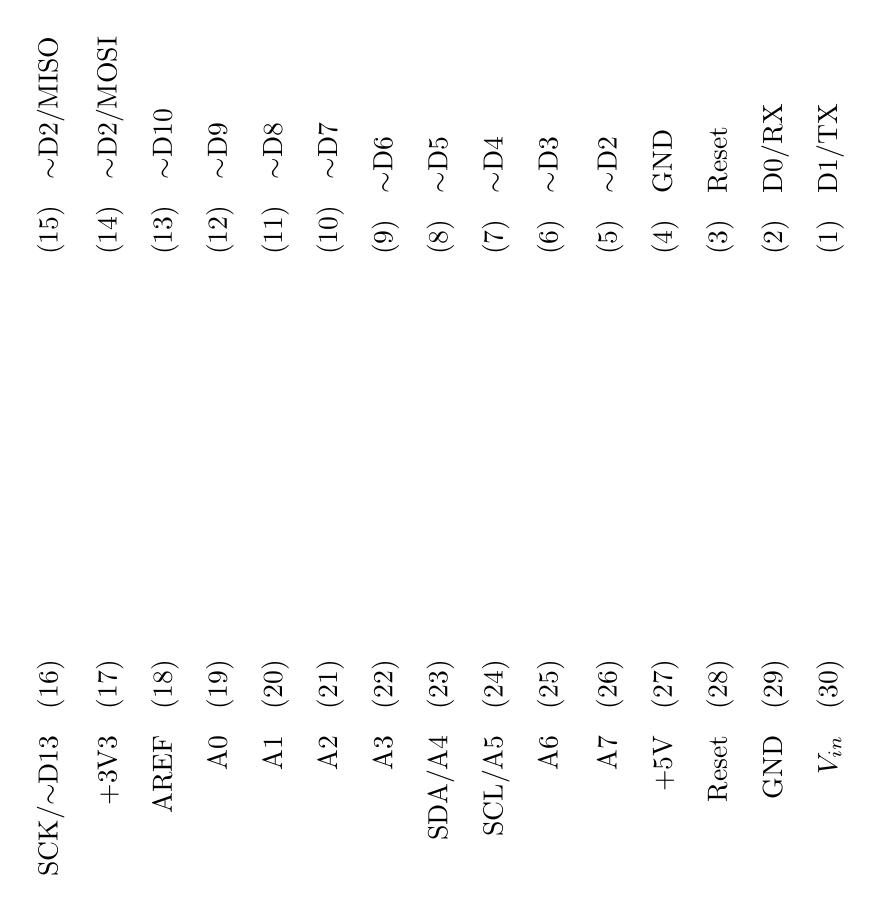
\begin{tikzpicture}
      
    \ArduinoNanoBLESenseRev

    \node[rotate=90,right] (Pin1) at (11.2,4.9) {(1) \; D1/TX};
    \node[rotate=90,right] (Pin2) at (10.5,4.9) {(2) \; D0/RX};
    \node[rotate=90,right] (Pin3) at (9.8,4.9) {(3) \; Reset};
    \node[rotate=90,right] (Pin4) at (9.1,4.9) {(4) \; GND};
    \node[rotate=90,right] (Pin5) at (8.4,4.9) {(5) \; $\sim$D2};
    \node[rotate=90,right] (Pin6) at (7.65,4.9) {(6) \; $\sim$D3};
    \node[rotate=90,right] (Pin7) at (6.95,4.9) {(7) \; $\sim$D4};
    \node[rotate=90,right] (Pin8) at (6.25,4.9) {(8) \; $\sim$D5};
    \node[rotate=90,right] (Pin9) at (5.55,4.9) {(9) \; $\sim$D6};
    \node[rotate=90,right] (Pin10) at (4.85,4.9) {(10) \; $\sim$D7};
    \node[rotate=90,right] (Pin11) at (4.15,4.9) {(11) \; $\sim$D8};
    \node[rotate=90,right] (Pin12) at (3.45,4.9) {(12) \; $\sim$D9};
    \node[rotate=90,right] (Pin13) at (2.75,4.9) {(13) \; $\sim$D10};
    \node[rotate=90,right] (Pin14) at (2.05,4.9) {(14) \; $\sim$D2/MOSI};
    \node[rotate=90,right] (Pin15) at (1.3,4.9) {(15) \; $\sim$D2/MISO};
    

    \node[rotate=90,left] (Pin30) at (11.2,-0.0) { $V_{in}$ \; (30)};
    \node[rotate=90,left] (Pin1) at (10.5,-0.0) {GND \; (29)};
    \node[rotate=90,left] (Pin2) at (9.8,-0.0) {Reset \; (28)};
    \node[rotate=90,left] (Pin3) at (9.1,-0.0) {+5V \; (27)};
    \node[rotate=90,left] (Pin4) at (8.4,-0.0) {A7 \; (26)};
    \node[rotate=90,left] (Pin5) at (7.65,-0.0) {A6 \; (25)};
    \node[rotate=90,left] (Pin6) at (6.95,-0.0) {SCL/A5 \; (24)};
    \node[rotate=90,left] (Pin7) at (6.25,-0.0) {SDA/A4 \; (23)};
    \node[rotate=90,left] (Pin8) at (5.55,-0.0) {A3 \; (22)};
    \node[rotate=90,left] (Pin9) at (4.85,-0.0) {A2 \; (21)};
    \node[rotate=90,left] (Pin10) at (4.15,-0.0) {A1 \; (20)};
    \node[rotate=90,left] (Pin11) at (3.45,-0.0) {A0 \; (19)};
    \node[rotate=90,left] (Pin12) at (2.75,-0.0) {AREF \; (18)};
    \node[rotate=90,left] (Pin13) at (2.05,-0.0) {+3V3 \; (17)};
    \node[rotate=90,left] (Pin14) at (1.3,-0.0) {SCK/$\sim$D13 \; (16)};

  \end{tikzpicture}
  \captionof{figure}[Pin assignment of the Arduino Nano 33 BLE Sense]{Pin assignment of the Arduino Nano 33 BLE Sense and for the Arduino Nano 33 BLE Sense Rev 2; note that the orange built-in LED is connected to pin D13 and the power LED to pin D1. The built-in RGB LED occupies pins D18, D19 and D20.}
\end{center}

\Mynote{Beide Diagramme}

\subsection{Gesture, Proximity, and Color Detection Sensor ADPS-9960}

The APDS-9960 device features advanced Gesture detection, Proximity detection, Digital Ambient Light Sense (ALS) and Color Sense (RGB). \cite{Arduino:2021} Gesture detection utilizes four directional photodiodes to sense reflected IR energy (sourced by the integrated LED) to convert physical motion information (i.e. velocity, direction and distance) to a digital information.

For the following Applications the sensor is in use:

\begin{itemize}
    \item Gesture Detection
    \item Color Sense
    \item Ambient Light Sensing
    \item Proximity Sensing
\end{itemize}

\subsection{Accelerometer, Gyroscope, and Magnetometre Sensor LSM9DS1}

The LSM9DS1 is a system-in-package featuring a 3D digital linear acceleration sensor, a 3D digital angular rate sensor, and a 3D digital magnetic sensor. \ac{imu}'s work by detecting rotational movements across the 3 axis known as Pitch, Roll and Yaw. To achieve the same, it depends on Accelerometer, Gyroscope and Magnetometer. The accelerometer gives the velocity at which the \ac{imu} module moves. The gyroscope measure the rotational movement rate on the \ac{imu}. Magnetometer measures the force of gravity acting on the \ac{imu}.

For the following Applications the \ac{imu} is in use:


\begin{itemize}
  \item Indoor navigation
  \item Advanced gesture recognition
  \item Gaming and virtual reality input devices
  \item Display/map orientation and browsing
  \item Consumer electronics; Smartphones, tablets, fitness trackers for motion sensing and orientation.
  \item Compact transportation solutions like Segway.
  \item Sports Technology - helping athletes to know how they can improve their movements.
\end{itemize}


There are also certain disadvantages of using the \ac{imu} and points that need to be kept in mind while using an \ac{imu} sensor. Accumulated error or \textit{'Drift'} is the main disadvantage of \ac{imu}s, present due to its constant measuring of changes and rounding off its calculated values off. When such a process happens for a prolonged period of time, it can lead to significant errors. The best way to avoid the \textit{drift} factor is to use a good quality \ac{imu} Sensor and make sure the \ac{imu} sensor is calibrated. \cite{STMicroelectronics:2015}
\Mynote{The explanation of drift is to small; citations}

\subsubsection{Calibration of an IMU}

\Mynote{What is calibration? citations!}

On research it was found that there are various methods to calibrate the sensors involved, the time period between each calibration is also not defined specifically, however it is advised that regular calibration is done especially when there are strange outputs noticed. Few methods of calibration are briefed below:

\subsubsection{Low and High Limit Method}

In this method the sensor is rotated in circles along each axis a few times. The midpoint is then found between the two extremes. If there is no offset, the midpoint is close to zero, but if there is a slight deviation from zero, this figure is the hard iron offset, which is the result of the distortion caused by the Earth's magnetic field. This method is mainly used to calibrate the Magnetometer \cite{Mallon:2015}

\subsubsection{Magneto V1.2}

In this method, the raw magnetometer data is pre-processed with axis specific gain correction to convert the raw output into nanoTesla: 

\begin{center} 
    
    \PYTHON{Xm\_nanoTesla = rawCompass.m.x*(100000.0/1100.0);}
    
    \PYTHON{Gain X [LSB/Gauss] for selected input field range}
    
    \PYTHON{Ym\_nanoTesla = rawCompass.m.y*(100000.0/1100.0);}
    
    \PYTHON{Zm\_nanoTesla = rawCompass.m.z*(100000.0/980.0);}
    
    
\end{center} 

This converted data is saved into the file  \FILE{Mag\_raw.txt} that you open with the Magneto program. To start using this method, we first need to replace the (100000.0/1100.0) scaling factors with values that convert your specific sensors output into nanoTesla. Rather than simply finding an offset and scale factor for each axis, Magneto creates twelve different calibration values that correct for a whole set of errors: bias, hard iron, scale factor, soft iron and misalignment.

A side benefit of this is that it can be used to calibrate accelerometers as well. You might again need to pre-process your specific raw accelerometer output, taking into account the bit depth and G sensitivity, to convert the data into milliGalileo. Then enter a value of 1000 milliGalileo as the ``norm'' for the gravitational field. \cite{Mallon:2015}




\Mynote{Here, we need more information because we want to use it:
\begin{itemize}
    \item General infomration about imus
    \item angle to roation matrix with example!
    \item calibration
    \item drift
    \item $\ldots$
    \item specials for this imu
    \item description of the parameters for coding
    \item example code, see Code/Nano33BLESense/IMU/Arduino
\end{itemize}
}

\subsection{Pressure Sensor LPS22HB}
The LPS22HB is an ultra-compact piezoresistive absolute pressure sensor which functions as a
digital output barometer.

For the following Applications the sensor is in use:



\begin{itemize}
    \item Altimeters and barometers for portable devices 
    \item Weather station equipment
    \item Sports watchs
\end{itemize}

A sensor element is installed as well as an IC interface that communicates via an I\textsuperscript{2}C or SPI bus. The function is given in a temperature range from $-40^\circ C$ to $+85^\circ C$. [STM17]

\begin{itemize}
  \item Absolutdruckbereich: 260 bis 1260 hPa
  \item Versorgungsspannung: 1,7 bis 3,6 Volt
  \item 24-bit Druckdatenausgabe
  \item 16-bit Temperaturdatenausgabe
\end{itemize}

\subsection{Relative Humidity and Temperature Sensor HTS221}
The HTS221 is an ultra-compact sensor for relative humidity and temperature. It includes a sensing element and a mixed signal to provide the measurement information through digital serial interfaces.

For the following Applications the sensor is in use:


\begin{itemize}
    \item Air conditioning, heating and ventilation 
    \item Air humidifiers
    \item Refrigerators
    \item Smart home automation
    \item Industrial automation
\end{itemize}  

Dieser Sensor kommuniziert über den I\textsuperscript{2}C- und SPI-Bus. Dieser Sensor ist einsetzbar in einem Temperaturbereich
von $-40^\circ C$ bis $+120^\circ C$. Zur Spannungsversorgung werden 1,7 bis 3,3 Volt benötigt. Eine Temperaturmessung erfolgt mit einer Genauigkeit von $\pm 5^\circ C$. [STM23]

\begin{itemize}
    \item GND - Ground
    \item DRDY - Data ready output signal
    \item SCL/SPC - I2C serial clocl (SCL) \& SPI serial port clock (SPC)
    \item VDD - Stromversorgung
    \item SDA/SDI/SDO - I\textsuperscript{2}C serial Data (SDA) \& 3 wire-SPI serial data input/output (SDI/SDO)
    \item SPI enable - I\textsuperscript{2}C/SPI mode selection
\end{itemize}

\subsection{Digital Microphone MP34DT05-A}

The MP34DT05-A is an ultra-compact, low-power, omni directional, digital microphone built with a capacitive sensing element and an IC interface. The sensing element, capable of detecting acoustic waves, is manufactured using a specialized silicon micromachining process dedicated to producing audio sensors.
The MP34DT05 is a low-distortion microphone with a signal-to-noise ratio of 64 dB. The sensitivity is -26 dBFS $\pm$ 3 dB. The \ac{aop} is 122.5 dBSPL.

The output signal of the microphone is a PDM signal. This signal is a binary signal modulated by \ac{pdm}  from the analogue signal. \cite{STMicroelectronics:2021}

For the following Applications the sensor is in use:

\begin{itemize}
    \item Speech recognition 
    \item Portable media player
    \item Mobile Terminal
\end{itemize}

\begin{figure}[h]
  
\includegraphics[width=16cm]{Microphon/MikrophonCP}
  \caption[Circuit diagram microphone]{Circuit diagram microphone \cite{STMicroelectronics:2021}}
\end{figure}

The Arduino nano 33 BLE Sense has a built-in microphone that uses PDM (Pulse-Density Modulation) to convert sound into digital data. You can use the PDM library to access the microphone data and perform various tasks with it. Here is a simple example of using the builtin microphone for an Arduino nano 33 BLE Sense:

\begin{code}
    \begin{Arduino}
        // Include the PDM library
        #include <PDM.h>
        
        // Buffer to store the microphone data
        short sampleBuffer[256];
        
        // Variable to store the sound level
        int soundLevel = 0;
        
        // Callback function for PDM data
        void onPDMdata() {
            // Read the PDM data
            int bytesAvailable = PDM.available();
            PDM.read(sampleBuffer, bytesAvailable);
            
            // Calculate the sound level
            soundLevel = 0;
            for (int i = 0; i < bytesAvailable / 2; i++) {
                soundLevel += abs(sampleBuffer[i]);
            }
            soundLevel /= bytesAvailable / 2;
        }
        
        void setup() {
            // Initialize serial communication
            Serial.begin(9600);
            while (!Serial);
            
            // Initialize PDM with a sample rate of 16 kHz and 16-bit resolution
            PDM.begin(1, 16000);
            PDM.onReceive(onPDMdata);
        }
        
        void loop() {
            // Print the sound level to the serial monitor
            Serial.println(soundLevel);
            delay(100);
        }
    \end{Arduino}
    \caption{Simple example using of the builtin microphone of the Arduino Nano 33 BLE Sense}\label{code:microphone}
\end{code}


The code~\ref{code:microphone} will print the sound level of the microphone to the serial monitor every 100 milliseconds. 

You can modify this code to perform other tasks with the microphone data, such as controlling LEDs, playing sounds, or sending data to other devices. For more information and examples, you can check out the PDM library documentation or the Arduino nano 33 BLE Sense page. 

\Mynote{How to install the library PDM\\description of the lib\\ functions}




\subsection{Bluetooth Module nRF52840}

The nRF52840 is an advanced, highly flexible single chip solution for today’s increasingly demanding Ultra Low Power (ULP) wireless applications for connected devices on our person, connected living environments and the \ac{iot} at large. It is designed ready for the major feature
advancements of Bluetooth 5 and takes advantage of Bluetooth 5's increased performance capabilities. \cite{Arduino:2021b}

\textbf{Applications}

\begin{itemize}
    \item Smart Home products
    \item Industrial mesh networks
    \item Smart city infrastructure
    \item Connected watches
    \item Advanced personal fitness devices
    \item Wearables with wireless payment
    \item Connected Health
\end{itemize}


\section{Bluetooth Module INA B306}

The module is a Bluetooth Low Energy (BLE). The connection with our smartphone is possible, to do this we have to use application ``Nordic Semiconductors nRF Connect'' They used 5.0 generation bluetooth. \ref{Figure:TestBluetoothConnect} 

\begin{center}
    \label{Figure:TestBluetoothConnect}
    
\includegraphics[width=10cm]{Bluetooth/connectionBLE.png}
    \captionof{figure}{Connection with BLE and smartphone}
\end{center}		

We can use for example to share Arduino batterie on smartphone, \ref{Code:TestBluetoothBattery} here you see an code example for how we can do this.

\begin{center}
    \captionof{figure}{Simple sketch to seen Arduino battery }
    \ArduinoExternal{}{../../Code/Nano33BLESense/Bluetooth/bluetooth.ino}
    \label{Code:TestBluetoothBattery}
\end{center}




\section{Arduino Nano 33 BLE Pin Configuration}

Arduino Nano 33 BLE is an advanced version of Arduino Nano board that is based on a powerful processor the nRF52840. The figure ~\ref{Schnittstellen} shows that the board has the following pin configuration. \href{https://www.etechnophiles.com/arduino-nano-33-ble-sense-pinout-introduction-specifications/}{Pin Configuration}


\begin{description}
  \item[Digital pin] The number of digital I/O pins are 14 which receive only two values HIGH or LOW. These pins can either be used as an input or output based on the requirement. When these pins receive 5V, they are in a HIGH state and when they receive 0V they are in a LOW state.
  \item[Analog pin] Total 8 analog pins available on the board A0 -- A7. These pins get any value as opposed to digital pins that only receive two values HIGH or LOW. These pins are used to measure the analog voltage ranging between 0 to 5V.
  \item[PWM pin] All digital pins can be used as PWM pins. These pins generate analog results with digital means.
  \item[SPI pin] The board supports serial peripheral interface (SPI) communication protocol. This protocol is employed to develop communication between a controller and other peripheral devices like shift registers and sensors. Two pins are used for SPI communication i.e. Master Input Slave Output (MISO) and Master Output Slave Input (MOSI) are used for SPI communication. These pins are used to send or receive data by the controller.
  \item[I2C pin] The board carries the I2C communication protocol which is a two-wire protocol. It comes with two pins SDL and SCL.
  \item[UART pin] The board features a UART communication protocol that is used for serial communication and carries two pins Rx and Tx. The Rx is a receiving pin used to receive the serial data while Tx is a transmission pin used to transmit the serial data.
  \item[External Interrupts pin] All digital pins can be used as external interrupts. This feature is used in case of emergency to interrupt the main running program with the inclusion of important instructions at that point.
  \item[LED at Pin 13 and AREF pin] There is an LED connected to pin 13 of the board. And AREF is a pin used as a reference voltage for the input voltage.
\end{description}



\begin{figure}[ht]
    \centering
    
\includegraphics[width=0.5\linewidth]{Nano33BLESense/Schnittstellen}
    \caption{Arduino Nano 33 BLE Pin Configuration}
    \label{Schnittstellen}
\end{figure}


\section{\textcolor{red}{Was fehlt}}

\textcolor{red}{
\begin{itemize}
  \item Beschreibung der Sensoren
    \begin{itemize}
      \item Hintergrundwissen
      \item Beschreibung
      \item Eigenschaften
      \item Kalibrierung
    \end{itemize}
  \item Beschreibung der Bibliothek
    \begin{itemize}
      \item Beschreibung
      \item Installation
      \item Funktionen
    \end{itemize}
  \item Laufzeit, Speicherplatz, \ldots
  \item Software-Dokumentation
  \item Verwendung von Werkzeugen, z.B. Doxygen
    \begin{itemize}
      \item Beschreibung, inklusive im Quellcode; z.B. Header
      \item Handbuch
      \item Ablaufdiagramm
      \item \ldots
\end{itemize}
\item Interpretation der Ergebnisse
\item Literatur, Bilder
\item \ldots
\end{itemize}
}


